% tech.tex -- running example for the semantic witness.
\documentclass[tikz,border=3pt]{standalone}
\usepackage[dvipsnames]{xcolor}
\usetikzlibrary{arrows.meta,positioning,calc}
\newcommand{\PredWR}{\mathsf{PredWR}}
\newcommand{\PredRW}{\mathsf{PredRW}}
\newcommand{\WW}{\mathsf{WW}}
\newcommand{\match}{\Delta}
\begin{document}
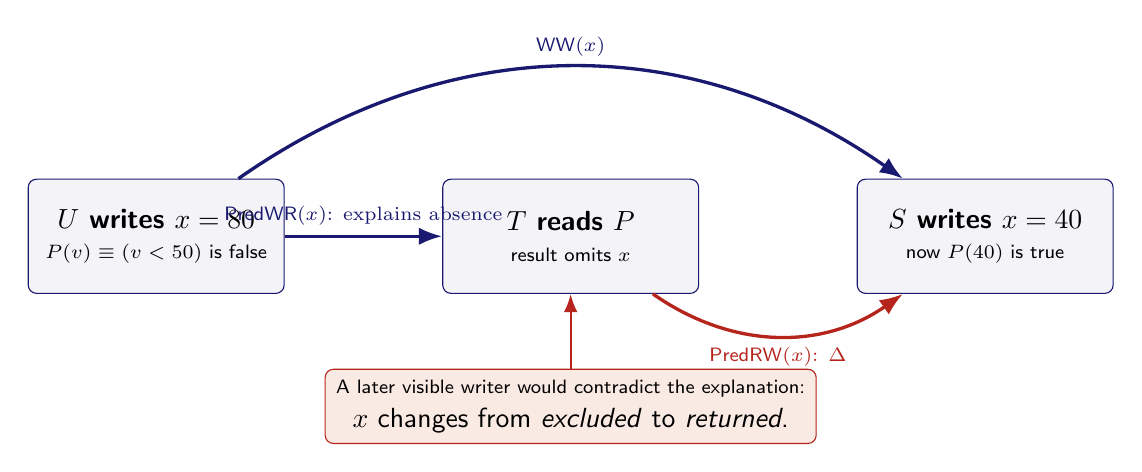
\begin{tikzpicture}[
  >=Latex,font=\sffamily,
  tx/.style={draw=MidnightBlue,rounded corners=3pt,fill=MidnightBlue!5,
    align=center,minimum width=3.25cm,minimum height=1.45cm,inner sep=4pt},
  note/.style={draw=BrickRed,rounded corners=3pt,fill=BrickRed!7,align=center,inner sep=4pt}]
  \node[tx] (u) {\textbf{$U$ writes $x=80$}\\[-1pt]\scriptsize $P(v)\equiv(v<50)$ is false};
  \node[tx,right=2.0cm of u] (t) {\textbf{$T$ reads $P$}\\[-1pt]\scriptsize result omits $x$};
  \node[tx,right=2.0cm of t] (s) {\textbf{$S$ writes $x=40$}\\[-1pt]\scriptsize now $P(40)$ is true};
  \draw[-Latex,very thick,MidnightBlue] (u) -- node[above,font=\scriptsize] {$\PredWR(x)$: explains absence} (t);
  \draw[-Latex,very thick,MidnightBlue] (u) to[bend left=35] node[above,font=\scriptsize] {$\WW(x)$} (s);
  \draw[-Latex,very thick,BrickRed] (t) to[bend right=35] node[below,font=\scriptsize] {$\PredRW(x)$: $\match$} (s);
  \node[note,below=.95cm of t] (note) {\scriptsize A later visible writer would contradict the explanation:\\
    $x$ changes from \emph{excluded} to \emph{returned}.};
  \draw[-Latex,thick,BrickRed] (note) -- (t.south);
\end{tikzpicture}
\end{document}
